In this section, we briefly discuss the main conclusions from our experiments and analysis in the form of recommendations for NLP practitioners.
We also discuss the general approach to dimensionality reduction from the point of view of distance learning and the limitations.
We summarize together with ideas for future work.

\section{Recommendations}

\subsection{Importance of Pre-/post-processing}

As our results show, for all methods (and models), centering and normalization should be done before and after dimension reduction, as it boosts the performance of every model.

\subsection{Method recommendation}

While most compression methods achieve similar retrieval performance and compression ratios (cf. \Cref{tab:retrieval_summary} and \Cref{tab:retrieval_summary_nq}), PCA stands out in the following regards:

\begin{itemize}
    \item It requires only minimal implementation effort and no tuning of hyper-parameters beyond selecting how many principal components to keep.
    \item As our analysis shows, the PCA matrix can be estimated well with only 1000 document or query embeddings. It is not necessary to learn a transformation matrix on the full knowledge base.
    \item PCA can easily be combined with precision reduction based approaches.
\end{itemize}

\subsection{Splitting}

Small gains (both performance and smaller knowledge base size) can be achieved by splitting on sentence boundaries (e.g. 6 sentences instead of 100 tokens).
Further improvements can be possibly made by using the same splitting scheme in model pretraining.

\section{Pitfalls of Reconstruction Loss} \label{sec:reconstruction_loss}

Despite PCA and autoencoder being the most successful methods, low reconstruction loss provides no theoretical guarantee to the retrieval performance.
Consider a simple linear projection that can be represented as a diagonal matrix that projects to a space of the same dimensionality.
This function has a trivial inverse and therefore no information is lost when it is applied.
The retrieval is however disrupted, as it will mostly depend on the first dimension and nothing else.
This is a major flaw of approaches that minimize the vector reconstruction loss because the optimized quantity is different to the actual goal.
\begin{gather*}
    R = \begin{pmatrix}
    10^{99} & 0 & {\cdots} & 0 \\
    0 & 1 & {\cdots} & 0 \\
    {\vdots}  & {\vdots}  & {\ddots} & {\vdots}  \\
    0 & 0 & {\cdots} & 1
    \end{pmatrix}
    \qquad
    R^{-1} = \begin{pmatrix}
    10^{-99} & 0 & {\cdots} & 0 \\
    0 & 1 & {\cdots} & 0 \\
    {\vdots}  & {\vdots}  & {\ddots} & {\vdots}  \\
    0 & 0 & {\cdots} & 1
    \end{pmatrix} \\ \\
    \forall v \in \mathbf{R}^d: L^2((R^{-1}\times R)v, v) = L^2(\text{I}v, v) = 0 \quad\Rightarrow\quad \mathcal{L} = 0
\end{gather*}

\subsection{Distance Learning}

In this subsection, we discuss a more general solution to dimension reduction for document retrieval: distance/manifold learning.
This task is also concerned with creating a new vector space that has some key properties transferred from the original, higher-dimensional, space (distances, ordering etc.).
\Cref{fig:manifold_example} illustrates dimension reduction on random vectors from 3D to 2D.\footnote{The 3D visualization is in itself a kind of dimension reduction but we add additional features (leading verticals and grid) to make use of the human visual processing.}
The various methods are discussed later.
Note the distances between the three selected points in the 2D space.

\begin{figure}[ht]
    \hspace{-0.05\linewidth}
    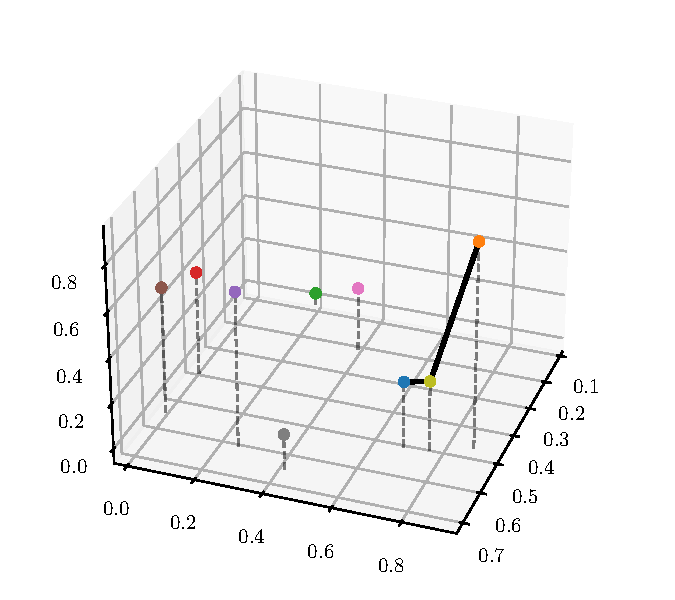
\includegraphics[width=0.58\linewidth]{img/manifold_examples_3d.pdf}
    \hspace{-0.06\linewidth}
    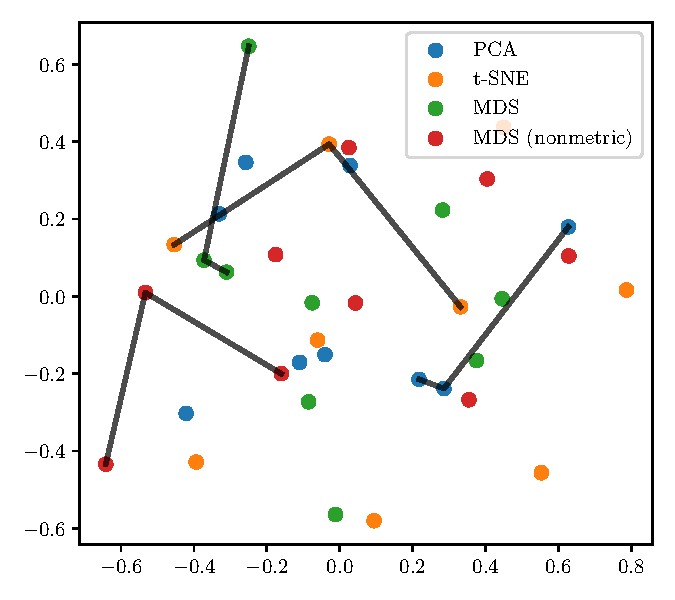
\includegraphics[width=0.54\linewidth]{img/manifold_examples_2d.pdf}
    \caption{Example of dimension reduction using PCA, t-SNE and parametric and non-parametric MDS from 3 to 2 dimensions.}
    \label{fig:manifold_example}
\end{figure}

\subsubsection{Existing Approaches}

The task of dimensionality reduction has been explored by standard statistical methods by the name manifold learning.

The most used method is t-distributed stochastic neighbor (t-SNE) embedding built on the work of \citet{hinton2002stochastic} or multidimensional scaling \citep{kruskal1964nonmetric,borg2005modern}.
They organize a new vector space (of lower dimensionality) so that the $L^2$ distances follow those of the original space (extensions to other metrics also exist).
Although the optimization goal is more in line with our task of vector space compression with the preservation of nearest neighbours, methods of manifold learning are limited by the large computation costs\footnote{
The common fast implementation for t-SNE, Barnes-Hut \citep{barnes1986hierarchical,van2013barnes} is based on either quadtrees or octrees and is limited to $3$ dimensions.} and the fact that they do not construct a function but rather move the discrete points in the new space to lower the optimization loss.
This makes it not applicable for online purposes (i.e. adding new samples that need to be compressed as well).

\paragraph{Multidimensional Scaling.}
A widely used technique for dimensionality reduction is MDS.
An extension to this is using an arbitrary metric for the original space, though the new organization is still based on the $L^2$ distance.
An important variant of this method is nonmetric MDS which preserves the ordering of neighbours instead of trying to model all distances accurately.
This optimization goal is important for the task at hand, dimensionality reduction for vectors used for document retrieval.
A downside of MDS is that the support is limited to metrics only in the formal mathematical sense, which the inner product does not satisfy and has very large computation costs.

\paragraph{Uniform Manifold Approximation and Projection for Dimension Reduction.}

While the recent technique UMAP \citep{mcinnes2018umap} solves some of the issues of t-SNE (target dimension limits), it is still too slow for practical purposes when applied to the whole knowledge base.

All of the manifold learning methods are also very dependent on the hyperparameters, which makes working with the techniques (in comparison to PCA) more difficult, also yielding suboptimal results.

\subsubsection{Gradient-based optimization}

The main disadvantage of the approaches based on reconstruction loss is that their optimization goal strays from what we are interested in, namely preserving distances between vectors.
% This is something that we explicitly try to capture in the method of similarity distillation.
We tried to reformulate the problem in terms of deep learning and gradient-based optimization to alleviate the issue of speed and extensibility of standard manifold learning approaches.
We try to learn a function that maps the original vector space to a lower-dimensional one while preserving similarities.
That can be either a simple linear projection $A$ or generally a more complex differentiable function $f$:
\begin{gather*}
\mathcal{L}=\text{MSE}(\text{sim}(f(t_i), f(t_j)), \text{sim}(t_i, t_j))
\end{gather*}

After the function $f$ is fitted, both the training and new data can be compressed by its application.
As opposed to manifold learning which usually leverages specific properties of the metrics, here they can be any differentiable functions.
The optimization was, however, too slow, underperforming (between sparse projection and PCA) and did not currently provide any benefits (results not shown in this thesis).

Similar to manifold learning, we may create completely new vectors instead of relying on differentiable transformations.
Given an already existing lower-dimensional representation of the data, we may consider the following loss, computed the gradient and updated the values.
Assuming $t_i$ and $t_j$ are randomly sampled vectors and the new vectors $n_i$ and $n_j$ are trainable parameters.
The elements in the pairs of vectors need not be from the same distribution. In this case, $t_i$ and $n_i$ may be queries and $t_j$ and $n_j$ documents.
The optimization goal is to have same similarities in the new vector space as in the original one.
\begin{gather*}
    \mathcal{L} = \text{MSE}(\text{sim}(n_i, n_j), \text{sim}(t_i, t_j))
\end{gather*}
    
Naturally, this is very susceptible to the initial organization of the vector space. We considered two solutions for initialization of every dimension: uniform sampling from $(-1,1)$ and sampling from a normal distribution with $\mu = 1$ and $\sigma^2 = 1$.
We also experimented with the normalization of the whole vector to the norm of $1$.
This method does not, however, solve the issue that the result of the computation is not applicable to new data and only reorganizes data at train-time.

We also tried to use unsupervised contrastive learning by considering close neighbours in the original space as positive samples and distant neighbours as negative samples but reached similar results:
\begin{gather*}
    \mathcal{L}= \frac{\sum_{t_i, t_j \text{ close}} e^{\text{sim}(f(t_i), f(t_j))}}{\sum_{t_i, t_j \text{ distant}} e^{\text{sim}(f(t_i), f(t_j))}}
\end{gather*}

\section{Limitation}

We are fairly confident, based on prior existing research on this topic, that the explored methods will not yield unexpected undesirable results.
We aimed at making deployment and experiments with large knowledge bases easier from compute and memory resrouces point of view.
A persisting bottleneck is the embedding model inference, which is required to generate the index for the whole knowledge base.
Additionally, for extremely resource limited scenarios, the application of these methods may not be straightforward.\footnote{For example, to avoid having the whole 150GB index in memory, one must interweave embedding model inference with dimension reduction steps.}

The key thing that could prevent from the described methods to be used by document retrieval practicioners is the lack of quantification of how the loss in retrieval performance affects the downstream task performance.
While we shown that there are no probably no systematic differences in the kinds of documents that are retrieved, it is still unknown whether 90\% of original retrieval performance means that a specific question answering system will have 90\% exact match.
Because this depends heavily on the specific task, we leave this question open for future survey and would like to see curves downstream task performance - retrieval retrieval performance for multiple systems and tasks.

\section{Summary} \label{sec:conclusion}

In this work, we examined several simple unsupervised methods for dimensionality reduction for retrieval-based NLP tasks: random projections, PCA, autoencoder and precision reduction and their combination.
We also documented the data requirements of each method and their reliance on pre- and post-processing.
We explored several options for splitting and filtering and reported that the commonly used practices are adequate.
We stress the importance of pre- and post-processing (centering + normalization).

\subsection*{Future research}

As shown in prior works, dimension reduction can take place also during training where the loss is more in-line with the retrieval goal.
Methods for dimension reduction after training, however, rely mostly on reconstruction loss, which is suboptimal.
Therefore more research for dimension reduction methods is needed, such as fast manifold or distance-based learning.

Despite negative results with gradient-based metric learning, we believe that with enough research, it may show to be useful.
It also leads to many new questions, for example, if the loss uses the inner product as the similarity in the new space and $L^2$ in the original, it is unclear to which extent the trained function would be able to capture the original $L^2$ structure with the inner product as the similarity metric.